\documentclass[10pt,letterpaper,twocolumn,twosided]{article}

\usepackage[utf8]{inputenc}
\usepackage[spanish]{babel}
\usepackage{listings}
\usepackage[usenames,dvipsnames]{color}
\usepackage{amsmath}
\usepackage{verbatim}
\usepackage{hyperref}
\usepackage{color}
\usepackage{geometry}

\geometry{verbose,landscape,letterpaper,tmargin=2cm,bmargin=2cm,lmargin=1cm,rmargin=1cm}
\newcommand{\codigofuente}[1]{
\verbatiminput{#1}
\dotfill
}

\setlength{\columnsep}{0.5in}
\setlength{\columnseprule}{1px}

\begin{document}

\title{Resumen de algoritmos para maratones de programación}
\author{Universidad Tecnológica de Pereira}
\maketitle

\tableofcontents
\lstloadlanguages{C++,Java}

%===============================================%
\section{Plantilla}

\codigofuente{src/template.cpp}

%===============================================%
\section{Grafos}

\subsection{Depth First Search}

Es un algoritmo para recorrer o buscar en un grafo. Empieza visitando la raiz y luego explora 
a fondo cada rama antes de hacer el backtraing.\\
\\
Complejidad $O(|V|+|E|)$

\codigofuente{src/graphs/dfs.cpp}

\subsection{Breadth First Search}

Es un algoritmo de búsqueda que empieza en la raíz y explora todos los nodos vecinos. Luego para cada
vecino repite el proceso hasta encontrar la meta.\\
Complejidad $O(|V|+|E|)$

\codigofuente{src/graphs/bfs.cpp}

\subsection{Shortest path problem}

El shortest path problem es el problema de encontrar el camino mas corto entre dos nodos de un grafo. Existen
dos algoritmos para solucionarlo: Dijkstra y Bellman-Ford. Si bien Dijkstra tiene una complejidad mejor que
Bellman-Ford, no funciona para grafos con aristas con peso negativo mientras que Bellman-Ford si lo hace.

\subsubsection{Dijkstra}

Calcula la ruta más corta a todos los nodos desde un origen.\\
Todas las aristas deben ser NO negativas, en ese caso usar Bellman-ford.\\
Complejidad $O(E\ log V)$

\codigofuente{src/graphs/dijkstra.cpp}


\subsubsection{Bellman-Ford}
Este algoritmo calcula la ruta más corta en un grafo dirigido, en el cual el peso de las aristas puede 
ser positivo o negativo. Para grafos con pesos NO-negativos, el algoritmo de Dijkstra resuelve más
rápido este problema.\\


Si un grafo contiene un ``Ciclo negativo'', por ejemplo, un ciclo cuya suma de aristas sea un valor negativo,
entonces camina de forma arbitraria con los pesos que puede ser construida, por ejemplo, no puede haber camino más corto.
El algoritmo puede detectar ciclos negativos y reportar su existencia, pero no puede producir una respuesta correcta
si un ciclo negativo es alcanzable desde el nodo origen.\\

Para solucionar el longest path, simplemente se aplica bellman-ford con los pesos de los caminos negativos.

\codigofuente{src/graphs/bellman.cpp}

\subsection{All-pairs shortest paths}

Es una versión del shortest path problem donde hay que hayar la menor distancia entre todos los nodos.

Existen dos algoritmos para solucionarlo, Floyd-Warshall y Jhonson. Floyd-Warshall lo hace en tiempo cúbico, 
mientras que Jhonson en $V x E$, por lo que solo es útil si $E$ es asimptoticamente menor que $V X V$ (es decir,
el grafo no es muy denso).

\subsubsection{Floyd-Warshall}

In computer science, the Floyd–Warshall algorithm (sometimes known as the WFI Algorithm or Roy–Floyd algorithm)
is a graph analysis algorithm for finding shortest paths in a weighted graph (with positive or negative edge weights).
A single execution of the algorithm will find the lengths (summed weights) of the shortest paths between all pairs
of vertices. The algorithm is an example of dynamic programming.

\codigofuente{src/graphs/floydwarshall.cpp}

\subsubsection{Johnson}

Johnson's algorithm is a way to find the shortest paths between all pairs of vertices in a
sparse directed graph. It allows some of the edge weights to be negative numbers, but no 
negative-weight cycles may exist. It works by using the Bellman–Ford algorithm to compute a
transformation of the input graph that removes all negative weights, allowing Dijkstra's algorithm 
to be used on the transformed graph.\\

Pseudocodigo:

Johnson's algorithm consists of the following steps:

First, a new node q is added to the graph, connected by zero-weight edges to each other node.\\

Second, the Bellman–Ford algorithm is used, starting from the new vertex q, to find for each vertex v the 
least weight h(v) of a path from q to v. If this step detects a negative cycle, the algorithm is terminated.\\

Next the edges of the original graph are reweighted using the values computed by the Bellman–Ford algorithm: 
an edge from u to v, having lengthw(u,v), is given the new length $ w(u,v) + h(u) - h(v).$\\

Finally, q is removed, and Dijkstra's algorithm is used to find the shortest paths from each node s to every
other vertex in the reweighted graph.\\

In the reweighted graph, all paths between a pair s and t of nodes have the same quantity $h(s) - h(t)$ added to
them, so a path that is shortest in the original graph remains shortest in the modified graph and vice versa.
However, due to the way the values h(v) were computed, all modified edge lengths are non-negative, ensuring the
optimality of the paths found by Dijkstra's algorithm. The distances in the original graph may be calculated from 
the distances calculated by Dijkstra's algorithm in the reweighted graph by reversing the reweighting transformation.\\

The time complexity of this algorithm, using Fibonacci heaps in the implementation of Dijkstra's algorithm, 
is O(V2log V + VE): the algorithm uses O(VE) time for the Bellman–Ford stage of the algorithm, and $O(V log V + E)$
for each of V instantiations of Dijkstra's algorithm. Thus, when the graph is sparse, the total time can be faster
than the Floyd–Warshall algorithm, which solves the same problem in time $ O(V3).$\\

\subsection{Minimum Spanning Tree}

Given a connected, undirected graph, a spanning tree of that graph is a subgraph which is a tree and connects all the vertices together. A single graph can have many different spanning trees. We can also assign a weight to each edge, which is a number representing how unfavorable it is, and use this to assign a weight to a spanning tree by computing the sum of the weights of the edges in that spanning tree. A minimum spanning tree (MST) or minimum weight spanning tree is then a spanning tree with weight less than or equal to the weight of every other spanning tree. More generally, any undirected graph (not necessarily connected) has a minimum spanning forest, which is a union of minimum spanning trees for its connected components.
One example would be a cable TV company laying cable to a new neighborhood. If it is constrained to bury the cable only along certain paths, then there would be a graph representing which points are connected by those paths. Some of those paths might be more expensive, because they are longer, or require the cable to be buried deeper; these paths would be represented by edges with larger weights. A spanning tree for that graph would be a subset of those paths that has no cycles but still connects to every house. There might be several spanning trees possible. A minimum spanning tree would be one with the lowest total cost.

Hay dos algoritmos para solucionar MST, Kruskal y Prim. Cada uno tiene sus ventajas y desventajas.

\subsubsection{Algoritmo de kruskal}

Kruskal's algorithm is an algorithm in graph theory that finds a minimum spanning tree for a connected weighted graph. This means it finds a subset of the edges that forms a tree that includes every vertex, where the total weight of all the edges in the tree is minimized. If the graph is not connected, then it finds a minimum spanning forest (a minimum spanning tree for each connected component). Kruskal's algorithm is an example of a greedy algorithm.

Where E is the number of edges in the graph and V is the number of vertices, Kruskal's algorithm can be shown to run in O(E log E) time, or equivalently, O(E log V) time, all with simple data structures. These running times are equivalent because:

E is at most V2 and logV2 = 2logV  is O(log V).
If we ignore isolated vertices, which will each be their own component of the minimum spanning forest, V <= E+1, so log V is O(log E).
We can achieve this bound as follows: first sort the edges by weight using a comparison sort in O(E log E) time; this allows the step "remove an edge with minimum weight from S" to operate in constant time. Next, we use a disjoint-set data structure (Union and Find) to keep track of which vertices are in which components. We need to perform O(E) operations, two find operations and possibly one union for each edge. Even a simple disjoint-set data structure such as disjoint-set forests with union by rank can perform O(E) operations in O(E log V) time. Thus the total time is O(E log E) = O(E log V).
Provided that the edges are either already sorted or can be sorted in linear time (for example with counting sort or radix sort), the algorithm can use more sophisticated disjoint-set data structure to run in O(E a(V)) time, where a is the extremely slowly-growing inverse of the single-valued Ackermann function.

\codigofuente{src/graphs/kruskal.cpp}

\subsubsection{Algoritmo de Prim}

Prim's algorithm is an algorithm that finds a minimum spanning tree for a connected weighted undirected graph. This means it finds a subset of the edges that forms a tree that includes every vertex, where the total weight of all the edges in the tree is minimized. Prim's algorithm is an example of a greedy algorithm. 

El algoritmo de Prim tiene exactamente el mismo tiempo de ejecución asimptotico que el de Dijkstra y usar una Fibonnaci Heap o una Binary Heap tienen los mismos beneficios.

\codigofuente{src/graphs/prim.cpp}

\subsection{Strongly Connected Components}

A directed graph is called strongly connected if there is a path from each vertex in the graph to every other vertex. In particular, this means paths in each direction; a path from a to b and also a path from b to a. The strongly connected components of a directed graph G are its maximal strongly connected subgraphs. 

If each strongly connected component is contracted to a single vertex, the resulting graph is a directed acyclic graph. A directed graph is acyclic if and only if it has no (nontrivial) strongly connected subgraphs (because a cycle is strongly connected, and every strongly connected graph contains at least one cycle).

\codigofuente{src/graphs/tarjanJava.cpp}

\subsection{Puntos de articulación}

%teoria

\codigofuente{src/graphs/puntos_articulacion.cpp}

\subsection{2-SAT}
para construir el grafo dirigido, se crea un nodo para cada variable y su negación, luego para cada disjunción se crean dos aristas asi:  desde la negación de la primera variable a la segunda, y de la negacion de la segunda variable a la primera, esto indica, que si no se puede cumplir una de las variables hay que cumplir la otra:
    (x0 | -x3) equiv (-x0 -> -x3) equiv (x3 -> x0)


In terms of the implication graph, two terms belong to the same strongly connected component whenever there exist chains of implications from one term to the other and vice versa. Therefore, the two terms must have the same value in any satisfying assignment to the given 2-satisfiability instance. In particular, if a variable and its negation both belong to the same strongly connected component, the instance cannot be satisfied, because it is impossible to assign both of these terms the same value.
\\
this is a necessary and sufficient condition: a 2-CNF formula is satisfiable if and only if there is no variable that belongs to the same strongly connected component as its negation.
\\
Their algorithm performs the following steps:

\begin{itemize}

\item Construct the implication graph of the instance, and find its strongly connected components using any of the known linear-time algorithms for strong connectivity analysis. (Tarjan)


\item Check whether any strongly connected component contains both a variable and its negation. If so, report that the instance is not satisfiable and halt.

\item Construct the condensation of the implication graph, a smaller graph that has one vertex for each strongly connected component, and an edge from component i to component j whenever the implication graph contains an edge uv such that u belongs to component i and v belongs to component j. The condensation is automatically a directed acyclic graph and, like the implication graph from which it was formed, it is skew-symmetric.

\item Topologically order the vertices of the condensation; the order in which the components are generated by Kosaraju's algorithm is automatically a topological ordering.

\item For each component in this order, if its variables do not already have truth assignments, set all the terms in the component to be false. This also causes all of the terms in the complementary component to be set to true.

\end{itemize}

\subsection{Maximum bipartite: Kuhn’s algorithm}
 There is a bipartite graph containing N vertices (n vertices in left part and k (N-n) vertices in right part of graph) and M edges. We are to find maximum bipartite matching, i.e. mark maximum number of edges, so that no one of them have adjacent vertices with each other.
 
 \codigofuente{src/graphs/kuhn.cpp}

\subsection{Flujo Máximo}
En términos de teoría de grafos, nos dan una red - un grafo dirigido, en donde cada arista tiene cierta capacidad c asociada a él, un vértice inicial (la fuente) y un vértice final (el sumidero). Se nos pide asociar otro valor f que satisfaga  $f  \leq c$ para cada arista de tal forma de que para cada vértice, diferente a la fuente y el sumidero, la suma de los valores asociados a las aristas que entran a él sea igual a la suma de los valores que salen. Se llamará f al flujo a través de la arista. Además se pide maximizar la suma de los valores asociados a los arcos que salen de la fuente, el cual es el flujo total en la red.

La funcion find path se puede implementar con un breadth first search, el cual garantiza que toma como maximo N x M/2 pasos, donde N es el numero de vertices y M es el numero de aristas de la red. También se puede implementar con un priority first search, para lo cual hay que definir una estructura nodo que tenga los atributes vertice, prioridad y vertice anterior en el camino. Se usa un arreglo bidimensional para guardar las capacidades de la red residual tras cada paso del algoritmo.

\codigofuente{src/graphs/maxflow.cpp}

\subsection{Lowest Common Ancestor}

The lowest common ancestor (LCA) is a concept in graph theory and computer science. Let T be a rooted tree with n nodes. The lowest common ancestor is defined between two nodes v and w as the lowest node in T that has both v and w as descendants (where we allow a node to be a descendant of itself).

The LCA of v and w in T is the shared ancestor of v and w that is located farthest from the root. Computation of lowest common ancestors may be useful, for instance, as part of a procedure for determining the distance between pairs of nodes in a tree: the distance from v to w can be computed as the distance from the root to v, plus the distance from the root to w, minus twice the distance from the root to their lowest common ancestor.

In a tree data structure where each node points to its parent, the lowest common ancestor can be easily determined by finding the first intersection of the paths from v and w to the root. In general, the computational time required for this algorithm is o(h) where h is the height of the tree (length of longest path from a leaf to the root). However, there exist several algorithms for processing trees so that lowest common ancestors may be found more quickly, in constant time per query after a linear time preprocessing stage.

In computer science, Tarjan's off-line least common ancestors algorithm (more precisely, least should actually be lowest) is an algorithm for computing lowest common ancestorsfor pairs of nodes in a tree, based on the union-find data structure. The lowest common ancestor of two nodes d and e in a rooted tree T is the node g that is an ancestor of both d and eand that has the greatest depth in T. It is named after Robert Tarjan, who discovered the technique in 1979. Tarjan's algorithm is offline; that is, unlike other lowest common ancestor algorithms, it requires that all pairs of nodes for which the lowest common ancestor is desired must be specified in advance. The simplest version of the algorithm uses the union find data structure, which unlike other lowest common ancestor data structures can take more than constant time per operation when the number of pairs of nodes is similar in magnitude to the number of nodes. A later refinement by Gabow and Tarjan (1983) speeds the algorithm up to linear time.

The pseudocode below determines the lowest common ancestor of each pair in P, given the root r of a tree in which the children of node n are in the set n.children. For this offline algorithm, the set P must be specified in advance. It uses the MakeSet, Find, and Union functions of a disjoint-set forest. MakeSet(u) removes u to a singleton set, Find(u) returns the standard representative of the set containing u, and Union(u,v) merges the set containing u with the set containing v. TarjanOLCA(r) is first called on the root r.

\codigofuente{src/graphs/tarjanOLCA.cpp}

\subsection{Topological sort}

In graph theory, a topological sort or topological ordering of a directed acyclic graph (DAG) is a linear ordering of its nodes in which each node comes before all nodes to which it has outbound edges. Every DAG has one or more topological sorts.
More formally, define the reachability relation R over the nodes of the DAG such that xRy if and only if there is a directed path from x to y. Then, R is a partial order, and a topological sort is a linear extension of this partial order, that is, a total order compatible with the partial order.

The usual algorithms for topological sorting have running time linear in the number of nodes plus the number of edges $(O(|V|+|E|))$.
One of these algorithms, first described by Kahn (1962), works by choosing vertices in the same order as the eventual topological sort. First, find a list of start nodes which have no incoming edges and insert them into a set S; at least one such node must exist if graph is acyclic. Then:

\codigofuente{src/graphs/toposort.cpp}

\subsection{Shortest pair of edge disjoint paths}

Edge disjoint shortest pair algorithm is an algorithm in computer network routing. The algorithm 
is used for generating the shortest pair of edge disjoint paths between a given pair of vertices as follows:\\

\begin{itemize}

\item Run the shortest pair algorithm for the given pair of vertices

\item Replace each edge of the shortest path (equivalent to two oppositely directed arcs) by a single arc directed 
towards the source vertex

\item Make the length of each of the above arcs negative

\item Run the shortest path algorithm (Note: the algorithm should accept negative costs)

\item Erase the overlapping edges of the two paths found, and reverse the direction of the remaining arcs on the 
first shortest path such that each arc on it is directed towards the sink vertex now. The desired pair of 
paths results.

\end{itemize}

\subsection{Shortest pair of completely disjoint paths}

In theoretical computer science and network routing, Suurballe's algorithm is an algorithm for finding two
disjoint paths in a nonnegatively-weighted directed graph, so that both paths connect the same pair of vertices
and have minimum total length. The algorithm was conceived by J. W. Suurballe and published in 1974. The main idea
of Surballe's algorithm is to use Dijkstra's algorithm to find one path, to modify the weights of the graph edges,
and then to run Dijkstra's algorithm a second time. The modification to the weights is similar to the weight 
modification in Johnson's algorithm, and preserves the non-negativity of the weights while allowing the second
instance of Dijkstra's algorithm to find the correct second path.

Suurballe's algorithm performs the following steps:

Find the shortest path tree T rooted at node s by running Dijkstra's algorithm. This tree contains for every vertex u,
a shortest path from s to u. Let P1 be the shortest cost path froms to t. The edges in T are called tree edges
and the remaining edges are called non tree edges.

Modify the cost of each edge in the graph by replacing the cost w(u,v) of every edge (u,v) 
by $w'(u,v) = w(u,v) - d(s,v) + d(s,u).$ According to the resulting modified cost function, all tree edges have a
cost of 0, and non tree edges have a non negative cost.

Create a residual graph Gt formed from G by removing the edges of G that are directed into s and by reversing 
the direction of the zero length edges along path P1.

Find the shortest path P2 in the residual graph Gt by running Dijkstra's algorithm.

Discard the reversed edges of P2 from both paths. The remaining edges of P1 and P2 form a subgraph with two 
outgoing edges at s, two incoming edges at t, and one incoming and one outgoing edge at each remaining vertex.
Therefore, this subgraph consists of two edge-disjoint paths from s to t and possibly some additional (zero-length)
cycles. Return the two disjoint paths from the subgraph.

\subsection{Eulerian path}

In graph theory, an Eulerian path is a path in a graph which visits each edge exactly once. Similarly, an Eulerian circuit is an Eulerian path which starts and ends on the same vertex. They were first discussed by Leonhard Euler while solving the famous Seven Bridges of Königsberg problem in 1736. Mathematically the problem can be stated like this:
Given the graph on the right, is it possible to construct a path (or a cycle, i.e. a path starting and ending on the same vertex) which visits each edge exactly once?
Euler proved that a necessary condition for the existence of Eulerian circuits is that all vertices in the graph have an even degree, and stated without proof that connected graphs with all vertices of even degree have an Eulerian circuit. The first complete proof of this latter claim was published in 1873 byCarl Hierholzer.[1]
The term Eulerian graph has two common meanings in graph theory. One meaning is a graph with an Eulerian circuit, and the other is a graph with every vertex of even degree. These definitions coincide for connected graphs.[2]
For the existence of Eulerian paths it is necessary that no more than two vertices have an odd degree; this means the Königsberg graph is not Eulerian. If there are no vertices of odd degree, all Eulerian paths are circuits. If there are exactly two vertices of odd degree, all Eulerian paths start at one of them and end at the other. Sometimes a graph that has an Eulerian path, but not an Eulerian circuit (in other words, it is an open path, and does not start and end at the same vertex) is called semi-Eulerian.

Properties

A connected undirected graph is Eulerian if and only if every graph vertex has an even degree.
An undirected graph is Eulerian if it is connected and can be decomposed into edge-disjoint cycles.
If an undirected graph G is Eulerian then its line graph L(G) is Eulerian too.
A directed graph is Eulerian if it is strongly connected and every vertex has equal in degree and out degree.
A directed graph is Eulerian if it is strongly connected and can be decomposed into edge-disjoint directed cycles.
An Eulerian path exists in a directed graph if and only if the graph's underlying undirected graph is connected, at most one vertex has out degree-in degree=1, at most one vertex has in degree-out degree=1 and every other vertex has equal in degree and out degree.
An undirected graph is traversable if it is connected and at most two vertices in the graph are of odd degree.

Constructing Eulerian paths and circuits

Consider a graph known to have all edges in the same component and at most two vertices of odd degree. We can construct an Eulerian path out of this graph by using Fleury's algorithm, which dates to 1883. We start with a vertex of odd degree—if the graph has none, then start with any vertex. At each step we move across an edge whose deletion would not disconnect the graph, unless we have no choice, then we delete that edge. At the end of the algorithm there are no edges left, and the sequence of edges we moved across forms an Eulerian cycle if the graph has no vertices of odd degree; or an Eulerian path if there are exactly two vertices of odd degree.

\section{Programación Dinámica}

\subsection{Edit Distance}

El edit distance entre dos cadenas está definido como el número mínimo de operaciones para convertir una cadena en otra
con tres operaciones, inserción, eliminación y reemplazo.\\
Nótese que $d[i - 1][j] + 1$ representa un costo de 1 para la inserción, $d[i][j - 1] + 1$ costo 1 para eliminación, y $d[i - 1][j - 1] + (s1[i - 1] == s2[j - 1] ? 0 : 1))$ representa costo 1 para reemplazo (en caso de que no sean iguales). Con estas concideraciones es fácil adaptar este problema a otros similares.

\codigofuente{src/dp/edit_distance.cpp}

\subsection{Integer Knapsack Problem}

The knapsack problem or rucksack problem is a problem in combinatorial optimization: Given a set of items, each with a weight and a value, determine the number of each item to include in a collection so that the total weight is less than or equal to a given limit and the total value is as large as possible.

\codigofuente{src/dp/knapsack.cpp}

\subsection{Counting Boolean Parenthesizations}

Dada una expresión booleana (por ejemplo true or false and true) se debe determinar cuántas maneras existen de agrupar las variables (poner paréntesis) de tal forma que la expresión sea verdadera.

\subsection{Longest Increasing Subsequence}

In computer science, the longest increasing subsequence problem is to find a subsequence of a given sequence in which the subsequence elements are in sorted order, lowest to highest, and in which the subsequence is as long as possible.

\codigofuente{src/dp/lis.cpp}

\subsection{Josephus problem}

In computer science and mathematics, the Josephus problem (or Josephus permutation) is a theoretical problem related to a certain counting-out game.
There are people standing in a circle waiting to be executed. After the first man is executed, certain number of people are skipped and one man is executed. Then again, people are skipped and a man is executed. The elimination proceeds around the circle (which is becoming smaller and smaller as the executed people are removed), until only the last man remains, who is given freedom.
The task is to choose the place in the initial circle so that you are the last one remaining and so survive.

\codigofuente{src/dp/josephus.cpp}

%===============================================%
\section{Matemáticas}

\subsection{Fórmulas útiles}

%%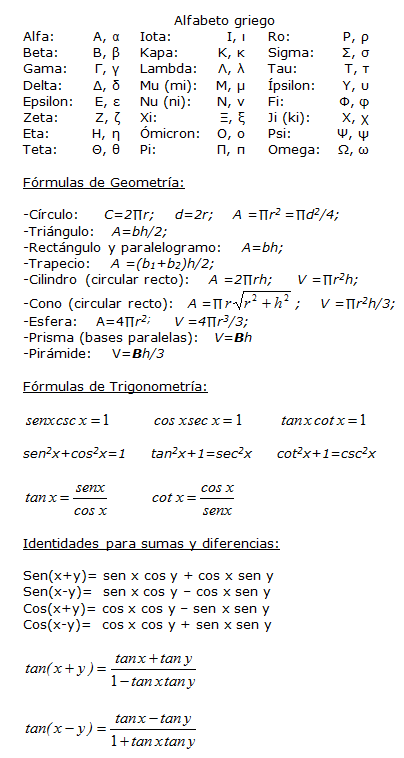
\includegraphics[height=12.4057cm,width=14.8205cm]{formulas1.jpg} %imagen.jpg es el nombre de la imagen que va a aparecer

\subsection{Aritmética Modular}

Colección de códigos útiles para aritmética modular\\

\codigofuente{src/mate/euclidean.cpp}

\subsection{Mayor exponente de un primo que divide a n!}

\codigofuente{src/mate/pow_div.cpp}

\subsection{Potencia modular}

\codigofuente{src/mate/mod_pow.cpp}

\subsection{Criba de Eratóstenes}

\codigofuente{src/mate/sieve.cpp}

\subsection{Test de primalidad}

\codigofuente{src/mate/rabin.cpp}


\subsection{Combinatoria}

\subsubsection{Sumas}

%\begin{tabular}{ l c r }

$$\sum_{k=0}^{n} k = \frac{n(n + 1)}{2}  $$\\ $$ \sum_{k=a}^{b} k = \frac{(a + b)(b - a + 1)}{2} $$ \\
$$ \sum_{k=0}^{n} k^2 = \frac{n(n + 1)(2n + 1)}{6} $$ \\ $$ \sum_{k=0}^{n} k^3 = \frac{n^{2}(n + 1)^{2}}{4} $$ \\
$$ \sum_{k=0}^{n} k^4 = \frac{(6n^5 + 15n^4 + 10n^3 - n)}{30} $$ \\ $$ \sum_{k=0}^{n} k^5 = \frac{(2n^6 + 6n^5 + 5n^4  - n^2)}{12} $$ \\
$$ \sum_{k=0}^{n} x^k = \frac{x^{n+1 - 1}}{x - 1} $$ \\

%%%===== REVISAR AQUI =======
$$ojo ! \sum_{k=0}^{n} kx^k = \frac{{x - {n + 1}x^{n+1} + nx^{n+2}}}{{x - 1} 1 + x + x^2 + \dots }= \frac{1}{{1 - x}} $$ \\
%\end{tabular}


\subsubsection{Cuadro Resumen}
Formulas para combinaciones y Permutaciones

\begin{tabular}[t]{|l |c |r|}
\hline
Tipo & ¿Se permite repeticion? & Fórmula \\
\hline
r permutaciones & No & $ {\frac{n!}{(n-r)!}} $ \\
\hline
r-combinaciones & No & $ {\frac{n!}{r!(n-r)!}} $  \\
\hline
r-permutaciones & Sí & $ {n^2} $ \\
\hline
r-combinaciones & Sí & ${\frac{(n+r-1)!}{r!(n-1)!}} $ \\
\hline
\end{tabular}

%===============================================%
\section{Geometría}

\subsection{Utilidades Geometría}
Código base para implementación de otros algoritmos.
\codigofuente{src/geom/utilities.cpp}

\subsection{Transformaciones}
\subsubsection{Rotación}
Para rotar un punto $(x,y)$ un ángulo $\theta$ (counterclockwise) con respecto al origen se tiene:

\[
 \begin{bmatrix}
  x \\
  y
 \end{bmatrix}
 =
 \begin{bmatrix}
  $cos(\theta)$ & $-sin(\theta)$ \\
  $sin(\theta)$ & $cos(\theta)$
 \end{bmatrix}
 *
 \begin{bmatrix}
  x \\
  y
 \end{bmatrix}
\]

Para rotar un punto $(x,y,z)$ un ángulo $\theta$ (counterclockwise) con respecto a un eje de rotación se tiene:($Rodrigues' rotation formula$)

\mathbf{v}_\mathrm{rot} = \mathbf{v} \cos\theta + (\mathbf{k} \times \mathbf{v})\sin\theta
  + \mathbf{k} (\mathbf{k} \cdot \mathbf{v}) (1 - \cos\theta).



\subsubsection{Desplazamiento dos dimensiones}
La traslacion es el efecto que conseguiremos al mover un objeto de un lugar a otro. Para lograrlo vamos a suponer un punto en algun lugar, ese punto u objeto tiene unas coordenas dadas en X y Y, muy bien ahora supongamos que queremos "trasladar" ese objeto a otro lugar a otra "coordenada", entonces lo que haremos sera :\\
Paso 1: Obtener el lugar donde se encuentra.\\
Paso 2: Dar a conocer cuantos lugares se movera, este dato sera en numeros enteros,es decir 1 espacio, 2 espacios, 3 espacios ó hasta n numero de espacios.\\
Luego hacemos lo siguiente:
\[
\left[ {\begin{array}{*{20}c}
   x & y & 1  \\
\end{array}} \right]\left[ {\begin{array}{*{20}c}
   1 & 0 & 0  \\
   0 & 1 & 0  \\
   {\Delta x} & {\Delta y} & 1  \\
\end{array}} \right] = \left[ {\begin{array}{*{20}c}
   {x + 0 + \Delta x} & {y + 0 + \Delta x} & {z + 0 + 0}  \\
\end{array}} \right]
\]


\subsection{Distancia mínima: Punto-Segmento}

\codigofuente{src/geom/minDistanceSgmntPnt.cpp}

\subsection{Distancia mínima: Punto-Recta}

\codigofuente{src/geom/punto_recta.cpp}

\subsection{Determinar si un polígono es convexo}

\codigofuente{src/geom/ifconvexpolygon.cpp}

\subsection{Determinar si un punto está dentro de un polígono convexo}

\codigofuente{src/geom/pointInaconvexpolygon.cpp}

\subsection{Determinar si un punto está dentro de un polígono cualquiera}

\codigofuente{src/geom/pointInAnyKindOfPolygon.cpp}

\subsection{Intersección de dos rectas}
Finds the intersection between two lines (Not segments! Infinite lines)\\
Line 1 passes through points (x0, y0) and (x1, y1).\\
Line 2 passes through points (x2, y2) and (x3, y3).\\
Handles the case when the 2 lines are the same (infinite intersections),\\
parallel (no intersection) or only one intersection.\\

\codigofuente{src/geom/intersectardosrectas.cpp}

\subsection{Intersección de dos segmentos}

\codigofuente{src/geom/inter_dos_segmentos.cpp}

\subsection{Determinar si dos segmentos se intersectan o no}

\codigofuente{src/geom/inter_dos_segmentos_si_no.cpp}

\subsection{Centro del círculo que pasa por tres puntos.}

\codigofuente{src/geom/centro_circulo_ters_puntos.cpp}

\subsection{Par de puntos más cercanos} 

An O(nlog n) algorithm for the closest pair problem, a divide and conquer approach. The main function \verb+closestpair+ receives the set of points ordered by x and y coordinates, in Px and Py, respectively.
WARNING: You must be careful with the algorithm used for splitting the points into two equal groups, it can produce endless recursive calls(Runtime error). The algorithm used here doesn't work when there are a lot of points with the same x coordinate, for solving this you must be sure that your algorithm always splits the group of points into two smaller groups of approximately equal size. 
 
\codigofuente{src/geom/closestpair.cpp}

\subsection{Par de puntos más alejados}

La función \verb+farthest_point_pair_distance+ encuentra la distancia mas grande que hay entre cualquier par de vértices de un polígono convexo (los puntos que se le pasan a la función deben estar ordenados clockwise) en $O(n)$ usando $rotating calipers$, por lo tanto si se quiere solucionar el problema de la distancia más grande entre cualquier par de puntos de una nube de puntos arbitraria se debe primero calcular el $convexhull$ de la nube de puntos y ejecutar este algoritmo sobre ese polígono para un complejidad total de $O(nlogn)$ si se usa un algoritmo eficiente para el $convexhull$.

\codigofuente{src/geom/farthest_point_pair_distance.cpp}

\subsection{Área de un polígono}

Si P es un polígono simple (no se intersecta a sí mismo) su área está dada
por:\\

$$ A(P) = \frac{1}{2} \sum_{i=0}^{n-1} (x_i*y_{i+1}-x_{i+1}*y_i)$$

P es un polígono ordenado anticlockwise.\\
Si es clockwise, retorna el area negativa.\\ 
Si no esta ordenado retorna basura.\\
P[0] != P[n-1]

\codigofuente{src/geom/areapoligono.cpp}

\subsection{Convexhull}

In mathematics, the convex hull or convex envelope for a set of points X in a real vector space V is the minimal convex set containing X.


In computational geometry, a basic problem is finding the convex hull for a given finite nonempty set of points in the plane. It is common to use the term "convex hull" for the boundary of that set, which is a convex polygon, except in the degenerate case that points are collinear. The convex hull is then typically represented by a sequence of the vertices of the line segments forming the boundary of the polygon, ordered along that boundary.

\subsubsection{Graham Scan}

\codigofuente{src/geom/convexhull.cpp}

\subsection{Great circle distance}

The great-circle distance or orthodromic distance is the shortest distance between any two points on the surface of a sphere measured along a path on the surface of the sphere (as opposed to going through the sphere's interior).

\codigofuente{src/geom/circledistance.cpp}

\subsection{Picks theorem}

Often we have to deal with polygons whose vertices have integer coordinates. Such polygons are called lattice polygons. Now, suppose we do not know the exact position of the vertices and instead we are given two values:

B = number of lattice points on the boundary of the polygon

I = number of lattice points in the interior of the polygon

Amazingly, the area of this polygon is then given by:

Area = B/2 + I - 1

The above formula is called Pick's Theorem due to Georg Alexander Pick (1859 - 1943). In order to show that Pick's theorem holds for all lattice polygons we have to prove it in 4 separate parts. In the first part we show that the theorem holds for any lattice rectangle (with sides parallel to axis). Since a right-angled triangle is simply half of a rectangle it is not too difficult to show that the theorem also holds for any right-angled triangle (with sides parallel to axis). The next step is to consider a general triangle, which can be represented as a rectangle with some right-angled triangles cut out from its corners. Finally, we can show that if the theorem holds for any two lattice polygons sharing a common side then it will also hold for the lattice polygon, formed by removing the common side. Combining the previous result with the fact that every simple polygon is a union of triangles gives us the final version of Pick's Theorem. Pick's theorem is useful when we need to find the number of lattice points inside a large polygon. 

Another formula worth remembering is Euler's Formula for polygonal nets. A polygonal net is a simple polygon divided into smaller polygons. The smaller polygons are called faces, the sides of the faces are called edges and the vertices of the faces are called vertices. Euler's Formula then states:
$V - E + F = 2$ , where

V = number of vertices
E = number of edges
F = number of faces
For example, consider a square with both diagonals drawn. We have V = 5, E = 8 and F = 5 (the outside of the square is also a face) and so V - E + F = 2. 

%===============================================%
\section{Strings}

\subsection{Knuth-Morris-Pratt KMP}

The Knuth–Morris–Pratt string searching algorithm (or KMP algorithm) searches for occurrences of a "word" W within a main "text string" S by employing the observation that when a mismatch occurs, the word itself embodies sufficient information to determine where the next match could begin, thus bypassing re-examination of previously matched characters.

\codigofuente{src/string/kmp.cpp}

\subsection{Aho-Corasick}

The Aho–Corasick string matching algorithm is a string searching algorithm invented by Alfred V. Aho and Margaret J. Corasick. It is a kind of dictionary-matching algorithm that locates elements of a finite set of strings (the "dictionary") within an input text. It matches all patterns simultaneously. The complexity of the algorithm is linear in the length of the patterns plus the length of the searched text plus the number of output matches. Note that because all matches are found, there can be a quadratic number of matches if every substring matches (e.g. dictionary = a, aa, aaa, aaaa and input string is aaaa).
Informally, the algorithm constructs a finite state machine that resembles a trie with additional links between the various internal nodes. These extra internal links allow fast transitions between failed pattern matches (e.g. a search for cat in a trie that does not contain cat, but contains cart, and thus would fail at the node prefixed by ca), to other branches of the trie that share a common prefix (e.g., in the previous case, a branch for attribute might be the best lateral transition). This allows the automaton to transition between pattern matches without the need for backtracking.
When the pattern dictionary is known in advance (e.g. a computer virus database), the construction of the automaton can be performed once off-line and the compiled automaton stored for later use. In this case, its run time is linear in the length of the input plus the number of matched entries.

\codigofuente{src/string/aho.cpp}

\subsection{Suffix Array}

In computer science, a suffix array is an array of integers giving the starting positions of suffixes of a string in lexicographical order.

\codigofuente{src/string/suffix_array.cpp}

\subsection{Minimum string rotation}

In computer science, the lexicographically minimal string rotation or lexicographically least circular substring is the problem of finding the rotation of a string possessing the lowest lexicographical order of all such rotations. For example, the lexicographically minimal rotation of "bbaaccaadd" would be "aaccaaddbb". It is possible for a string to have multiple lexicographically minimal rotations, but for most applications this does not matter as the rotations must be equivalent. Finding the lexicographically minimal rotation is useful as a way of normalizing strings. If the strings represent potentially isomorphic structures such as graphs, normalizing in this way allows for simple equality checking. A common implementation trick when dealing with circular strings is to concatenate the string to itself instead of having to perform modular arithmetic on the string indices.

\codigofuente{src/string/minrot.cpp}

%===============================================%
\section{Teoría de Juegos}

%===============================================%
\section{Estructuras de Datos}

\subsection{RMQ}

Range Minimum Query (RMQ) is used on arrays to find the position of an element with the minimum value between two specified indices. We will see later that the LCA problem can be reduced to a restricted version of an RMQ problem, in which consecutive array elements differ by exactly 1.
However, RMQs are not only used with LCA. They have an important role in string preprocessing, where they are used with suffix arrays (a new data structure that supports string searches almost as fast as suffix trees, but uses less memory and less coding effort). 

\codigofuente{src/structures/rmq.cpp}

\subsection{Union-find (disjoint-set)}

Union Find is an algorithm which uses a disjoint-set data structure to solve the following problem: Say we have some number of items. We are allowed to merge any two items to consider them equal (where equality here obeys all of the properties of an Equivalence Relation). At any point, we are allowed to ask whether two items are considered equal or not.
Definition

Basically a Union Find data structure implements two functions:

union( A, B ) - merge A's set with B's set

find( A ) - finds what set A belongs to

This is a common way to find connectivity between nodes, or to find connected components.

\codigofuente{src/structures/uf.cpp}


\subsection{Prefix Tree - Triee}

The tries can insert and find strings in $O(L)$ time (where L represent the length of a single word). This is much faster than set , but is it a bit faster than a hash table.


\codigofuente{src/structures/trie.cpp}


\subsection{Fenwick Tree}

Fenwick tree (aka Binary indexed tree) is a data structure that maintains a sequence of elements, and is able to compute cumulative sum of any range of consecutive elements in $O(logn)$ time. Changing value of any single element needs O(logn) time as well.
The structure is space-efficient in the sense that it needs the same amount of storage as just a simple array of n elements.

\codigofuente{src/structures/fenwick.cpp}

\subsection{Interval Tree}

%===============================================%
\section{Hashing} %%http://eternallyconfuzzled.com/tuts/algorithms/jsw_tut_hashing.aspx

\subsection{FNV Hash}

\codigofuente{src/hashing/FNV.cpp}

\subsection{JSW Hash}
Este es el más recomendado en términos de distribución.
\codigofuente{src/hashing/JSW.cpp}

%===============================================%
\section{Miseláneo}

\subsection {Bitwise operations}
Operaciones útiles con bits.

Use the following formula to turn off the rightmost 1-bit in a word, producing
0 if none (e.g., 01011000 becomes 01010000):

$$x \& (x - 1)$$

Use the following formula to isolate the rightmost 0-bit, producing 0 if none
(e.g., 10100111 becomes 00001000):

$$ not(x) \& (x + 1)$$

Use the following formula to right-propagate the rightmost 1-bit, producing
all 1’s if  (e.g., 01011000 becomes 01011111):

$$ x | (x - 1 )$$

Use the following formula to turn off the rightmost contiguous string of 1-bits
(e.g., 01011000 becomes 01000000):

$$ ((x | (x - 1 )) + 1 ) \& x$$

\codigofuente{src/bitwise.cpp}

\subsection{Física}

\subsubsection{Movimiento parabólico} 
estas son algunas ecuaciones del movimiento parabólico que pueden ser útiles:
la velocidad en x es constante y la aceleración gravitacional apunta hacia la tierra.\\

velocidad en y: $ vs_{y} = v_{0y} +(-g)*t   $\\ 
posición en x:  $ x = v_{0x}*t   $\\
posición en y:  $ y = y_{0} + v_{0y}*t + 1/ $ \\

\subsection{Stable marriage}

In mathematics, the stable marriage problem (SMP) is the problem of finding a stable matching between two sets of elements given a set of preferences for each element. A matching is a mapping from the elements of one set to the elements of the other set. A matching is stable whenever it is not the case that both:
some given element A of the first matched set prefers some given element B of the second matched set over the element to which A is already matched, and
B also prefers A over the element to which B is already matched
In other words, a matching is stable when there does not exist any alternative pairing (A, B) in which both A and B are individually better off than they would be with the element to which they are currently matched.
The problem is commonly stated as:
Given n men and n women, where each person has ranked all members of the opposite sex with a unique number between 1 and n in order of preference, marry the men and women together such that there are no two people of opposite sex who would both rather have each other than their current partners. If there are no such people, all the marriages are "stable".

In 1962, David Gale and Lloyd Shapley proved that, for any equal number of men and women, it is always possible to solve the SMP and make all marriages stable. They presented analgorithm to do so.[1][2]
The Gale-Shapley algorithm involves a number of "rounds" (or "iterations") where each unengaged man "proposes" to the most-preferred woman to whom he has not yet proposed. Each woman then considers all her suitors and tells the one she most prefers "Maybe" and all the rest of them "No". She is then provisionally "engaged" to the suitor she most prefers so far, and that suitor is likewise provisionally engaged to her. In the first round, first a) each unengaged man proposes to the woman he prefers most, and then b) each woman replies "maybe" to her suitor she most prefers and "no" to all other suitors. In each subsequent round, first a) each unengaged man proposes to the most-preferred woman to whom he has not yet proposed (regardless of whether the woman is already engaged), and then b) each woman replies "maybe" to her suitor she most prefers (whether her existing provisional partner or someone else) and rejects the rest (again, perhaps including her current provisional partner). The provisional nature of engagements preserves the right of an already-engaged woman to "trade up" (and, in the process, to "jilt" her until-then partner).

This algorithm guarantees that:

Everyone gets married 

Once a woman becomes engaged, she is always engaged to someone. So, at the end, there cannot be a man and a woman both unengaged, as he must have proposed to her at some point (since a man will eventually propose to everyone, if necessary) and, being unengaged, she would have to have said yes.

The marriages are stable 

Let Alice be a woman and Bob be a man who are both engaged, but not to each other. Upon completion of the algorithm, it is not possible for both Alice and Bob to prefer each other over their current partners. If Bob prefers Alice to his current partner, he must have proposed to Alice before he proposed to his current partner. If Alice accepted his proposal, yet is not married to him at the end, she must have dumped him for someone she likes more, and therefore doesn't like Bob more than her current partner. If Alice rejected his proposal, she was already with someone she liked more than Bob.

\codigofuente{src/misc/stable.cpp}

\subsection{Poker}

\codigofuente{src/misc/poker.cpp}

\subsection{Inversions}

Inversion Count for an array indicates – how far (or close) the array is from being sorted. If array is already sorted then inversion count is 0. If array is sorted in reverse order that inversion count is the maximum.

Formally speaking, two elements a[i] and a[j] form an inversion if a[i] > a[j] and i < j

Example:

The sequence 2, 4, 1, 3, 5 has three inversions (2, 1), (4, 1), (4, 3).

\codigofuente{src/misc/inversions.cpp}

\subsection{Nim}

Nim is a two-player mathematical game of strategy in which players take turns removing objects from distinct heaps. On each turn, a player must remove at least one object, and may remove any number of objects provided they all come from the same heap.
Variants of Nim have been played since ancient times. The game is said to have originated in China (it closely resembles the Chinese game of "Jianshizi", or "picking stones"), but the origin is uncertain; the earliest European references to Nim are from the beginning of the 16th century. Its current name was coined by Charles L. Bouton of Harvard University, who also developed the complete theory of the game in 1901, but the origins of the name were never fully explained. The name is probably derived from German nimm meaning "take", or the obsolete English verb nim of the same meaning. It should also be noted that rotating the word NIM by 180 degrees results in WIN (see Ambigram).
Nim is usually played as a misère game,[citation needed] in which the player to take the last object loses. Nim can also be played as a normal play game, which means that the person who makes the last move (i.e., who takes the last object) wins. This is called normal play because most games follow this convention, even though Nim usually does not.
Normal play Nim (or more precisely the system of nimbers) is fundamental to the Sprague-Grundy theorem, which essentially says that in normal play every impartial game is equivalent to a Nim heap that yields the same outcome when played in parallel with other normal play impartial games (see disjunctive sum).
While all normal play impartial games can be assigned a nim value, that is not the case under the misère convention. Only tame games can be played using the same strategy as misère nim.

A normal play game may start with heaps of 3, 4 and 5 objects:

In order to win always leave an even total number of 1's, 2's, and 4's.

Sizes of heaps  Moves\\
A B C\\
 
3 4 5           Player 1 takes 2 from A\\
1 4 5           Player 2 takes 3 from C\\
1 4 2           Player 1 takes 1 from B\\
1 3 2           Player 2 takes 1 from B\\
1 2 2           Player 1 takes entire A heap, leaving two 2s.\\
0 2 2           Player 2 takes 1 from B\\
0 1 2           Player 1 takes 1 from C leaving two 1s. (In misère play I would take 2 from C leaving (0, 1, 0).)\\
0 1 1           Player 2 takes 1 from B\\
0 0 1           Player 1 takes entire C heap and wins.\\

Mathematical theory

Nim has been mathematically solved for any number of initial heaps and objects; that is, there is an easily calculated way to determine which player will win and what winning moves are open to that player. In a game that starts with heaps of 3, 4, and 5, the first player will win with optimal play, whether the misère or normal play convention is followed.
The key to the theory of the game is the binary digital sum of the heap sizes, that is, the sum (in binary) neglecting all carries from one digit to another. This operation is also known as "exclusive or" (xor) or "vector addition over GF(2)". Within combinatorial game theory it is usually called the nim-sum, as will be done here. The nim-sum of x and y is written x * y to distinguish it from the ordinary sum, x + y. An example of the calculation with heaps of size 3, 4, and 5 is as follows:

Binary  Decimal\\
 
  0112    310    Heap A\\
  1002    410    Heap B\\
  1012    510    Heap C\\
  ---\\
  0102    210    The nim-sum of heaps A, B, and C, 3 * 4 * 5 = 2\\

An equivalent procedure, which is often easier to perform mentally, is to express the heap sizes as sums of distinct powers of 2, cancel pairs of equal powers, and then add what's left:

3 = 0 + 2 + 1 =     2   1      Heap A\\
4 = 4 + 0 + 0 = 4              Heap B\\
5 = 4 + 0 + 1 = 4       1      Heap C\\
---\\
2 =                 2          What's left after canceling 1s and 4s\\

In normal play, the winning strategy is to finish every move with a Nim-sum of 0. This is always possible if the Nim-sum is not zero before the move. If the Nim-sum is zero, then the next player will lose if the other player does not make a mistake. To find out which move to make, let X be the Nim-sum of all the heap sizes. Take the Nim-sum of each of the heap sizes with X, and find a heap whose size decreases. The winning strategy is to play in such a heap, reducing that heap to the Nim-sum of its original size with X. In the example above, taking the Nim-sum of the sizes is X = 3 * 4 * 5 = 2. The Nim-sums of the heap sizes A=3, B=4, and C=5 with X=2 are
(* representa xor)
A * X = 3 * 2 = 1 [Since (011) * (010) = 001 ]\\
B * X = 4 * 2 = 6\\
C * X = 5 * 2 = 7\\
The only heap that is reduced is heap A, so the winning move is to reduce the size of heap A to 1 (by removing two objects).
As a particular simple case, if there are only two heaps left, the strategy is to reduce the number of objects in the bigger heap to make the heaps equal. After that, no matter what move your opponent makes, you can make the same move on the other heap, guaranteeing that you take the last object.
When played as a misère game, Nim strategy is different only when the normal play move would leave no heap of size 2 or larger. In that case, the correct move is to leave an odd number of heaps of size 1 (in normal play, the correct move would be to leave an even number of such heaps).
In a misère game with heaps of sizes 3, 4 and 5, the strategy would be applied like this:

A B C Nim-sum\\
 
3 4 5 0102=210   I take 2 from A, leaving a sum of 000, so I will win.\\
1 4 5 0002=010   You take 2 from C\\
1 4 3 1102=610   I take 2 from B\\
1 2 3 0002=010   You take 1 from C\\
1 2 2 0012=110   I take 1 from A\\
0 2 2 0002=010   You take 1 from C\\
0 2 1 0112=310   The normal play strategy would be to take 1 from B, leaving an even number (2)\\
                 heaps of size 1.  For misère play, I take the entire B heap, to leave an odd\\
                 number (1) of heaps of size 1.\\
0 0 1 0012=110   You take 1 from C, and lose.\\

\subsection{Sudoku}

\codigofuente{src/misc/sudoku.cpp}

\codigofuente{src/misc/sudokuE.cpp}

\subsection{Gaussian elimination}

\codigofuente{src/misc/gaussian.cpp}

\subsection{Catalan numbers}

In combinatorial mathematics, the Catalan numbers form a sequence of natural numbers that occur in various counting problems, often involving recursively defined objects. They are named after the Belgian mathematician Eugène Charles Catalan (1814–1894).

The Nth catalan number is given by:

$$C_n = {2n\choose n} - {2n\choose n+1} \quad\text{ for }n\ge 0$$

Cn is the number of Dyck words of length 2n. A Dyck word is a string consisting of n X's and n Y's such that no initial segment of the string has more Y's than X's (see also Dyck language). For example, the following are the Dyck words of length 6:

$$XXXYYY \;\;\;   XYXXYY  \;\;\;  XYXYXY  \;\;\;  XXYYXY   \;\;\;  XXYXYY$$.

Re-interpreting the symbol X as an open parenthesis and Y as a close parenthesis, Cn counts the number of expressions containing n pairs of parentheses which are correctly matched:

$$((()))   \;\;\;  ()(())    \;\;\; ()()()   \;\;\;  (())()   \;\;\;  (()())$$

Cn is the number of different ways n + 1 factors can be completely parenthesized (or the number of ways of associating n applications of a binary operator).

Successive applications of a binary operator can be represented in terms of a full binary tree. (A rooted binary tree is full if every vertex has either two children or no children.) It follows that Cn is the number of full binary trees with n + 1 leaves.

If the leaves are labelled, we have the quadruple factorial numbers.

Cn is the number of non-isomorphic ordered trees with n+1 vertices. (An ordered tree is a rooted tree in which the children of each vertex are given a fixed left-to-right order.)

Cn is the number of monotonic paths along the edges of a grid with n x n square cells, which do not pass above the diagonal. A monotonic path is one which starts in the lower left corner, finishes in the upper right corner, and consists entirely of edges pointing rightwards or upwards. Counting such paths is equivalent to counting Dyck words: X stands for move right and Y stands for move up.

Cn is the number of different ways a convex polygon with n + 2 sides can be cut into triangles by connecting vertices with straight lines.

Cn is the number of stack-sortable permutations of {1, ..., n}. A permutation w is called stack-sortable if S(w) = (1, ..., n), where S(w) is defined recursively as follows: write w = unv where n is the largest element in w and u and v are shorter sequences, and set S(w) = S(u)S(v)n, with S being the identity for one-element sequences. These are the permutations that avoid the pattern 231.

Cn is the number of permutations of {1, ..., n} that avoid the pattern 123 (or any of the other patterns of length 3); that is, the number of permutations with no three-term increasing subsequence. For n = 3, these permutations are 132, 213, 231, 312 and 321. For n = 4, they are 1432, 2143, 2413, 2431, 3142, 3214, 3241, 3412, 3421, 4132, 4213, 4231, 4312 and 4321.

Cn is the number of noncrossing partitions of the set {1, ..., n}. A fortiori, Cn never exceeds the nth Bell number. Cn is also the number of noncrossing partitions of the set {1, ..., 2n} in which every block is of size 2. The conjunction of these two facts may be used in a proof by mathematical induction that all of the free cumulants of degree more than 2 of the Wigner semicircle law are zero. This law is important in free probability theory and the theory of random matrices.

Cn is the number of ways to tile a stairstep shape of height n with n rectangles.

Cn is the number of standard Young tableaux whose diagram is a 2-by-n rectangle. In other words, it is the number ways the numbers 1, 2, ..., 2n can be arranged in a 2-by-n rectangle so that each row and each column is increasing. As such, the formula can be derived as a special case of the hook-length formula.

Cn is the number of ways that the vertices of a convex 2n-gon can be paired so that the line segments joining paired vertices do not intersect.

Cn is the number of semiorders on n unlabeled items.

\subsection{Bell numbers}

In combinatorics, the nth Bell number, named after Eric Temple Bell, is the number of partitions of a set with n members, or equivalently, the number of equivalence relations on it. Starting with B0 = B1 = 1, the first few Bell numbers are:

1, 1, 2, 5, 15, 52, 203, 877, 4140, 21147, 115975

The Bell numbers satisfy this recursion formula:

$$B_{n+1}=\sum_{k=0}^{n}{{n \choose k}B_k}.$$

\subsection{Polinomios}

\codigofuente{src/misc/polynomials.cpp}

\end{document}
